\documentclass[12pt, a4paper]{book}

\usepackage[T1]{fontenc}
\usepackage[utf8]{inputenc}
\usepackage[charter, cal=cmcal]{mathdesign}
\usepackage[scaled=0.92]{helvet}
\usepackage{geometry}
\geometry{a4paper, top=30mm, bottom=30mm, inner=32mm, outer=25mm, marginparwidth=18mm}

\usepackage{amsmath, amsthm}
\usepackage[version=4]{mhchem}
\usepackage{graphicx}
\usepackage{xcolor}
\usepackage{tikz}
\usetikzlibrary{arrows.meta, shapes.geometric, positioning, calc, backgrounds}
\usepackage{pgfplots}
\pgfplotsset{compat=1.18}
\usepackage{tcolorbox}
\tcbuselibrary{skins, breakable, theorems}
\usepackage{titlesec}
\usepackage{fancyhdr}
\usepackage{enumitem}
\usepackage{booktabs}
\usepackage{array}
\usepackage{parskip}
\usepackage{siunitx}
\usepackage[colorlinks=true, linkcolor=BrickRed,
            urlcolor=NavyBlue, citecolor=ForestGreen]{hyperref}

% ── Colours (Charcoal / Royal Blue) ──────────────────────────────────────────
\definecolor{JourneyColor}{HTML}{0F172A}
\definecolor{ModuleColor}{HTML}{2563EB}
\definecolor{PuzzleColor}{HTML}{D97706}
\definecolor{DiscoveryColor}{HTML}{3B82F6}
\definecolor{WarningColor}{HTML}{991B1B}
\definecolor{ProblemColor}{HTML}{6B21A8}
\definecolor{ReflectColor}{HTML}{0D9488}
\definecolor{HistoryColor}{HTML}{78350F}

% ── Boxes ─────────────────────────────────────────────────────────────────────
\newtcolorbox{puzzlebox}[1][]{enhanced,breakable,
  colback=PuzzleColor!6,colframe=PuzzleColor,fonttitle=\bfseries\sffamily,
  title={The Puzzle},attach boxed title to top left={yshift=-2mm,xshift=6mm},
  boxed title style={colback=PuzzleColor},borderline west={3pt}{0pt}{PuzzleColor},#1}

\newtcolorbox{discoverybox}[1][]{enhanced,breakable,
  colback=DiscoveryColor!8,colframe=DiscoveryColor,fonttitle=\bfseries\sffamily,
  title={Discovery},attach boxed title to top left={yshift=-2mm,xshift=6mm},
  boxed title style={colback=DiscoveryColor},borderline west={3pt}{0pt}{DiscoveryColor},#1}

\newtcolorbox{problembox}[1][]{enhanced,breakable,
  colback=ProblemColor!5,colframe=ProblemColor,fonttitle=\bfseries\sffamily,
  title={Problems},attach boxed title to top left={yshift=-2mm,xshift=6mm},
  boxed title style={colback=ProblemColor},borderline west={3pt}{0pt}{ProblemColor},#1}

\newtcolorbox{deepbox}[1][]{enhanced,breakable,
  colback=JourneyColor!5,colframe=JourneyColor,fonttitle=\bfseries\sffamily,
  title={Deep Problems},attach boxed title to top left={yshift=-2mm,xshift=6mm},
  boxed title style={colback=JourneyColor},borderline west={4pt}{0pt}{JourneyColor},#1}

\newtcolorbox{historybox}[1][]{enhanced,breakable,
  colback=HistoryColor!7,colframe=HistoryColor!60,fonttitle=\bfseries\sffamily\small,
  title={Historical Note},attach boxed title to top left={yshift=-2mm,xshift=6mm},
  boxed title style={colback=HistoryColor!80},#1}

\newtcolorbox{reflectionbox}[1][]{enhanced,breakable,
  colback=ReflectColor!6,colframe=ReflectColor,fonttitle=\bfseries\sffamily,
  title={Reflection},attach boxed title to top left={yshift=-2mm,xshift=6mm},
  boxed title style={colback=ReflectColor},borderline west={3pt}{0pt}{ReflectColor},#1}

\newtcolorbox{namedconcept}[2][]{enhanced,
  colback=ModuleColor!6,colframe=ModuleColor,fonttitle=\bfseries\sffamily\large,
  title={#2},attach boxed title to top left={yshift=-2mm,xshift=6mm},
  boxed title style={colback=ModuleColor},#1}

% ── Section formatting ────────────────────────────────────────────────────────
\titleformat{\chapter}[display]
  {\normalfont\sffamily\huge\bfseries\color{JourneyColor}}
  {\textcolor{JourneyColor!60}{\chaptertitlename\ \thechapter}}{10pt}{\Huge}
  [\vspace{2pt}\textcolor{JourneyColor}{\titlerule[1.5pt]}]
\titleformat{\section}
  {\normalfont\sffamily\Large\bfseries\color{ModuleColor}}
  {\thesection}{1em}{}[\textcolor{ModuleColor!40}{\titlerule[0.6pt]}]
\titleformat{\subsection}
  {\normalfont\sffamily\large\bfseries\color{JourneyColor!80}}{\thesubsection}{1em}{}
\titleformat{\subsubsection}
  {\normalfont\sffamily\normalsize\bfseries}{\thesubsubsection}{1em}{}

\pagestyle{fancy}
\fancyhf{}
\fancyhead[LE]{\small\sffamily\textcolor{JourneyColor}{\leftmark}}
\fancyhead[RO]{\small\sffamily\textcolor{ModuleColor}{\rightmark}}
\fancyfoot[C]{\small\thepage}
\renewcommand{\headrulewidth}{0.4pt}

\newcommand{\newterm}[1]{\textit{\textcolor{DiscoveryColor}{#1}}}
\newcommand{\important}[1]{\textcolor{ModuleColor}{\textbf{#1}}}

\begin{document}

\setcounter{chapter}{4}
\chapter[Journey 5 --- Algorithms, Data Structures, and Optimization]
        {Journey Five\\[8pt]
         \textcolor{ModuleColor}{\large Algorithms, Data Structures, and Optimization}}
\setcounter{section}{1}

\section{Module 5.2 --- Advanced Data Structures and Balanced Trees}
\label{sec:mod5.2}

\subsection*{Motivation}

We completed in Module 5.1 the asymptotic scaling limits of algorithms, proving that comparison-based sorting is bounded by $\Omega(n \log n)$.
But sorting is only useful if we have structured ways to store and query data dynamically.
We must study the geometry of storage.

If we insert sorted keys into a basic Binary Search Tree (BST), the tree collapses into a slow, linear list of $O(n)$ search complexity.
To maintain logarithmic $O(\log n)$ search times under arbitrary insertions, we must use self-balancing trees.
This module explores **AVL** and **Red-Black trees**, formalizing the rotation mechanics that restore balance dynamically.
Then, we will transition to **Hashing**, analyzing collision resolution strategies and universal hashing families that guarantee constant $O(1)$ expected search times.

\subsection{The Balance Problem}

We analyze the instability of unconstrained binary search trees.

\begin{puzzlebox}
\textbf{The Collapsed Search Tree.}

Suppose we store a list of $n$ distinct names in a Binary Search Tree (BST).
\begin{enumerate}[label=(\alph*), leftmargin=*]
  \item If the names arrive in random order, the tree grows relatively evenly.
        Explain why the expected search complexity for any key is $O(\log n)$ in this balanced state.
  \item Now, suppose the names arrive in alphabetical order.
        Draw the resulting BST.
        Show why the height of this tree collapses to $h = n$, making search complexity degenerate to linear $O(n)$.
  \item To prevent this, **AVL trees** enforce the balance invariant: for any node, the height difference between its left and right subtrees (the **Balance Factor**) can be at most 1.
        Suppose we have a tree of height 2 that becomes unbalanced after inserting a key:
        \begin{center}
        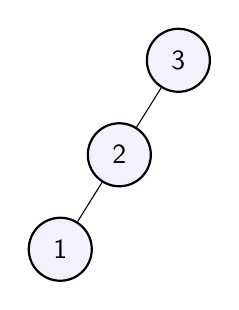
\begin{tikzpicture}[
          level distance=1.2cm,
          sibling distance=1.5cm,
          node/.style={circle, draw, thick, fill=blue!5, minimum size=0.8cm, font=\sffamily}
        ]
          \node[node] {3}
            child { node[node] {2}
              child { node[node] {1} }
              child[missing]
            }
            child[missing];
        \end{tikzpicture}
        \end{center}
        Show how a single **Right Rotation** around node 3 restores balance, producing a tree of height 1.
\end{enumerate}
\end{puzzlebox}

\subsection{Self-Balancing Red-Black Trees}

We formalize the coloring invariants that bound binary search tree heights.

\begin{namedconcept}{Red-Black Tree Properties}
A \newterm{Red-Black Tree} is a binary search tree where every node is colored either red or black, satisfying:
1. Every node is either **Red** or **Black**.
2. The **Root** is Black.
3. Every leaf ($\text{NIL}$ pointer) is Black.
4. If a node is Red, then both its children are Black (no consecutive Red nodes).
5. For each node, all simple paths from the node to descendant leaves contain the same number of black nodes (the **black-height**, $bh(x)$).
\end{namedconcept}

\begin{explobox}
These properties guarantee that no path from the root to a leaf is more than twice as long as any other path, ensuring the tree remains balanced.
\begin{enumerate}[label=(\alph*), leftmargin=*]
  \item Why does Property 4 prevent two red nodes from appearing in series on any path?
  \item If a path has black-height $bh = 3$, what is the minimum possible physical length (number of edges) of this path? What is the maximum possible physical length? (Consider the placement of red nodes).
  \item Prove that the path from the root to the deepest leaf is at most twice as long as the path to the shallowest leaf.
\end{enumerate}
\end{explobox}

\subsection{Hash Tables and Universal Hashing}

We study constant-time data access and the mathematics of collision prevention.

\begin{explobox}
Caches and lookup directories require faster access than trees. We map keys directly to table slots using a **Hash Function** $h: U \to \{0, \dots, m-1\}$.
* **Collisions:** Occur when $h(x) = h(y)$ for $x \neq y$. We resolve collisions by **chaining** (linked lists at each slot) or **open addressing** (searching alternative slots).
* **Load Factor ($\alpha$):** Defined as $\alpha = n/m$, representing the average number of keys per table slot.
\begin{enumerate}[label=(\alph*), leftmargin=*]
  \item Under the assumption of simple uniform hashing, prove that the expected time to search for a key in a hash table with chaining is $\Theta(1 + \alpha)$.
  \item An adversary can choose keys that all hash to the same slot, making the search time degenerate to $O(n)$.
        To prevent this, we select $h$ at random from a **Universal Family** $\mathcal{H}$.
        A family $\mathcal{H}$ of hash functions is universal if for any distinct keys $x, y \in U$:
        \[
          \Pr_{h \in \mathcal{H}} [h(x) = h(y)] \;\le\; \frac{1}{m}.
        \]
        Why does universal hashing make it impossible for an adversary to force worst-case collisions?
\end{enumerate}
\end{explobox}

\newpage

% ─── Section: Discovery ──────────────────────────────────────────────────────
\section{Part 3 --- Discovery}

\begin{discoverybox}
\textbf{What have we built?}

\textbf{First.} Basic BSTs can collapse to $O(n)$ linear complexity under sorted inputs, requiring balancing strategies.

\textbf{Second.} AVL trees enforce strict height invariants using local single and double rotations to restore balance factors.

\textbf{Third.} Red-Black trees use coloring rules to guarantee that the tree height is bounded by $h \le 2 \log_2(n+1)$, maintaining $O(\log n)$ search times.

\textbf{Fourth.} Universal Hashing randomly selects functions from a family where collision probability is bounded by $1/m$, ensuring $O(1)$ expected search times.
\end{discoverybox}

\newpage

% ─── Section: Naming Concepts ────────────────────────────────────────────────
\section{Part 4 --- What This Is Called}

\begin{namedconcept}{Data structure parameters}
* **AVL Tree:** Adelson-Velsky and Landis tree. A strictly self-balancing binary search tree.
* **Red-Black Tree:** A self-balancing binary search tree utilizing color properties.
* **Black-Height ($bh(x)$):** The number of black nodes on any path from node $x$ to a leaf, excluding $x$.
* **Universal Hashing:** A randomized hashing strategy using families of functions with bounded collision probabilities.
* **Load Factor ($\alpha$):** The ratio of keys to slots in a hash table, scaling collision rates.
\end{namedconcept}

\newpage

% ─── Section: Solved Exercises ───────────────────────────────────────────────
\section{Part 5 --- Solved Exercises}

\begin{problembox}
\begin{enumerate}[label=\textbf{E\arabic*.}]
  \item \textbf{Single Left Rotation on AVL Tree.}
  
        Show the single left rotation operation on a 3-node right-skewed BST to restore its AVL balance factor.
        
        \textbf{Solution:}
        Let us start with the unbalanced right-skewed tree:
        \begin{center}
        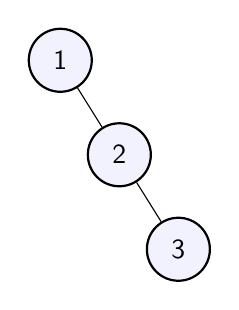
\begin{tikzpicture}[
          level distance=1.2cm,
          sibling distance=1.5cm,
          node/.style={circle, draw, thick, fill=blue!5, minimum size=0.8cm, font=\sffamily}
        ]
          \node[node] {1}
            child[missing]
            child { node[node] {2}
              child[missing]
              child { node[node] {3} }
            };
        \end{tikzpicture}
        \end{center}
        * The balance factor of node 1 is $height(left) - height(right) = 0 - 2 = -2$ (unbalanced).
        * We execute a **Single Left Rotation** around node 1.
          * Node 2 becomes the new root.
          * Node 1 becomes the left child of node 2.
          * Node 3 remains the right child of node 2.
        
        The rotated balanced tree:
        \begin{center}
        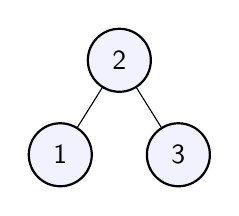
\begin{tikzpicture}[
          level distance=1.2cm,
          sibling distance=1.5cm,
          node/.style={circle, draw, thick, fill=blue!5, minimum size=0.8cm, font=\sffamily}
        ]
          \node[node] {2}
            child { node[node] {1} }
            child { node[node] {3} };
        \end{tikzpicture}
        \end{center}
        The balance factor of the new root is $height(left) - height(right) = 1 - 1 = 0$, satisfying the AVL constraint.
        
  \item \textbf{Path Invariant Proof in Red-Black Trees.}
  
        Prove that in a Red-Black tree, the path from the root to the deepest leaf is at most twice as long as the path to the shallowest leaf.
        
        \textbf{Solution:}
        Let $P_{\text{short}}$ be the shortest path from the root to any leaf, and $P_{\text{long}}$ be the longest path.
        * Let $bh(root)$ be the black-height of the root.
        * By Property 5 of Red-Black trees, every path from the root to a leaf contains the exact same number of black nodes.
        * Therefore, the number of black nodes on both $P_{\text{short}}$ and $P_{\text{long}}$ is equal to $bh(root)$.
        
        1. **Shortest path bound:**
           The shortest possible path occurs if the path contains only black nodes.
           \[
             |P_{\text{short}}| \;\ge\; bh(root).
           \]
        2. **Longest path bound:**
           By Property 4, a red node cannot have a red child. This means red nodes cannot be adjacent.
           Thus, the maximum number of red nodes we can insert in a path is at most equal to the number of black nodes.
           So, the longest path can contain at most $bh(root)$ red nodes in addition to the $bh(root)$ black nodes:
           \[
             |P_{\text{long}}| \;\le\; 2 \cdot bh(root).
           \]
        3. **Combine the inequalities:**
           Combine (1) and (2):
           \[
             |P_{\text{long}}| \;\le\; 2 \cdot bh(root) \;\le\; 2 \cdot |P_{\text{short}}|.
           \]
        Thus, the longest path is at most twice the length of the shortest path, guaranteeing the tree remains balanced.
\end{enumerate}
\end{problembox}

\newpage

% ─── Section: Problems ───────────────────────────────────────────────────────
\section{Part 6 --- Problems}

\begin{problembox}
\begin{enumerate}[label=\textbf{P\arabic*.}]
  \item \textbf{Red-Black Tree Insertion.}
  
        Draw the Red-Black tree resulting from inserting the keys $10, 20, 30, 15$ sequentially into an empty tree.
        Specify:
        \begin{enumerate}[label=(\alph*)]
          \item The color of each node after each insertion.
          \item Any rotation and recoloring operations executed to restore the Red-Black invariants.
        \end{enumerate}

  \item \textbf{Double Hashing Collision Resolution.}
  
        We hash keys into a hash table of size $m = 11$ using double hashing:
        \[
          h(k, i) \;=\; \left( h_1(k) + i \cdot h_2(k) \right) \bmod 11,
        \]
        where:
        * $h_1(k) = k \bmod 11$.
        * $h_2(k) = 1 + (k \bmod 10)$.
        \begin{enumerate}[label=(\alph*)]
          \item Insert the keys $22, 33, 44, 12$ sequentially. Show the occupied slots and any collision resolution probes.
          \item Explain why double hashing is superior to linear probing ($h_2(k) = 1$) in preventing **primary clustering** (where long runs of filled slots build up, slowing down search).
        \end{enumerate}
\end{enumerate}
\end{problembox}

\newpage

% ─── Section: Deep Problems ──────────────────────────────────────────────────
\section{Part 7 --- Deep Problems}

\begin{deepbox}
\begin{enumerate}[label=\textbf{D\arabic*.}]
  \item \textbf{Height Upper Bound Proof for Red-Black Trees.}
  
        We prove that a Red-Black tree with $n$ internal nodes has height $h \le 2 \log_2(n+1)$.
        
        \begin{enumerate}[label=(\alph*)]
          \item Prove by induction that the subtree rooted at any node $x$ contains at least $2^{bh(x)} - 1$ internal nodes, where $bh(x)$ is the black-height of $x$.
                *(Hint: For the base case, if $x$ is a leaf, $bh(x) = 0$, and it contains $2^0 - 1 = 0$ internal nodes. For the induction step, analyze the two children of $x$. How does their black-height compare to $bh(x)$?)*
          \item By Property 4, at least half of the nodes on any path from the root to a leaf (excluding the root) must be black.
                Use this to show that the black-height of the root satisfies:
                \[
                  bh(root) \;\ge\; \frac{h}{2}.
                \]
          \item Combine the results of (a) and (b) to show:
                \[
                  n \;\ge\; 2^{bh(root)} - 1 \;\ge\; 2^{h/2} - 1.
                \]
                Solve this inequality for $h$ to prove that $h \le 2 \log_2(n+1)$.
        \end{enumerate}

  \item \textbf{Expected Collision Count in Universal Hashing.}
  
        Let $h$ be chosen at random from a universal family $\mathcal{H}$ of hash functions mapping key universe $U$ to $\{0, \dots, m-1\}$.
        Let $S \subseteq U$ be a subset of keys of size $|S| = n$.
        For any key $x \in S$, let $C_x$ be the random variable representing the number of collisions with other keys in $S$:
        \[
          C_x \;=\; \sum_{y \in S, y \neq x} X_{xy},
        \]
        where $X_{xy}$ is the indicator random variable: $X_{xy} = 1$ if $h(x) = h(y)$, and $0$ otherwise.
        
        \begin{enumerate}[label=(\alph*)]
          \item Using the definition of universal hashing, write down the expected value $E[X_{xy}]$ for any $x \neq y$.
          \item Using the linearity of expectation, prove that:
                \[
                  E[C_x] \;\le\; \frac{n-1}{m} \;<\; \alpha,
                \]
                where $\alpha = n/m$ is the load factor.
          \item Why does this result guarantee that the expected search time for *any* key is bounded by $O(1)$ under universal hashing, regardless of the choice of keys?
        \end{enumerate}
\end{enumerate}
\end{deepbox}

\newpage

% ─── Section: Reflection ─────────────────────────────────────────────────────
\section{Part 8 --- Reflection}

\begin{reflectionbox}
\textbf{Conceptual Reflection}

Consider the following questions:
\begin{enumerate}
  \item **On the Balance of Invariants:** AVL trees enforce strict balance factors, requiring many rotations during writes. Red-Black trees relax the balance constraints, reducing write latency at the cost of slightly longer search paths. How does this choose between read-heavy and write-heavy workloads in software systems?
  \item **On the Role of Entropy:** Universal Hashing prevents worst-case collisions by selecting a hash function at random. How does introducing this probabilistic choice protect our data structures from malicious attacks (like Hash DoS attacks)?
  \item **On Hashing vs. Trees:** Hashing provides fast $O(1)$ expected search times, but loses the ordered structure of the keys. Trees maintain $O(\log n)$ search while keeping keys sorted (enabling range queries). How does this illustrate the fundamental engineering trade-off between *speed* and *order*?
\end{enumerate}
\end{reflectionbox}

\medskip
\noindent\textbf{Looking ahead.}
Module~5.3 introduces **Graph Algorithms and Network Flow**. Having mastered the storage and retrieval of individual keys, we will study relationships between elements: graphs, pathfinding (Dijkstra, Bellman-Ford), and flow networks (Ford-Fulkerson).

\vspace{1.4cm}
\begin{center}
{\color{JourneyColor}\rule{0.5\linewidth}{0.8pt}}\\[6pt]
{\small\color{JourneyColor}\textit{End of Journey 5, Module 5.2 --- Advanced Data Structures and Balanced Trees}}\\[4pt]
{\small\color{JourneyColor}Continue to: \textbf{Module 5.3 --- Graph Algorithms and Network Flow}}\\[6pt]
{\color{JourneyColor}\rule{0.5\linewidth}{0.8pt}}
\end{center}

\end{document}
